\chapter{KiemConfigurationPlugin}
\label{chapter:KiemConfig}
\begin{itemize}
 \item own plugin for modularity, reuse of old code, no interference with other plugins
\end{itemize}

\section{Extension Point Implementation}
\subsection{Implementing Classes}
\begin{itemize}
 \item toolbar provider: link to contribution manager, forward array of contributions
 \item configuration provider: link to configuration manager, forward requests
 \item event listener: handles events received by the configData component 
    listen to load/save events, can be disabled when KIEMConf is about to trigger load/save
\end{itemize}

\subsection{Manager Classes}
\begin{itemize}
 \item bundled control behavior 
 \item no cluttering up the main activator class
 \item singleton pattern
\end{itemize}
\subsubsection{Abstract Manager Superclass}
\begin{itemize}
 \item provides methods that all managers need
 \item load/save through the plugins preference store
 \item add/remove/notify listeners
\end{itemize}

\subsubsection{Schedule Manager}
\begin{itemize}
 \item all schedule data
 \item track recently used schedule Ids
 \item ask KIEMPlugin to load a saved schedule, deal with error
 \item add/remove schedules, update schedule priorities
 \item handle user load/save events
\end{itemize}

\subsubsection{Configuration Manager}
\begin{itemize}
 \item manages current/default configuration, supply filtered lists for preference components
 \item find current configuration and wrapper in data component wrapper list 
 \item get values for properties (where to look, ignored keys, save to current when found)
  \begin{itemize}
   \item check if there is a current configuration, check if the key is not on the ignored key list, try to find in current configuration
   \item on failure: try to find in default configuration, update current configuration, return found value
   \item on failure: if default value supplied, update default configuration, update current configuration, return default value
   \item on failure: throw exception
  \end{itemize}
 \item add/remove properties, update values
 \begin{itemize}
  \item try to update saved values
  \item if it doesn't exist create it
 \end{itemize}
 \item restore default values
\end{itemize}

\subsubsection{Editor Manager}
\begin{itemize}
 \item all editor definitions
 \item add/remove/find editors
 \item default editors 
\end{itemize}

\subsubsection{Other Managers}
\begin{itemize}
 \item contribution manager: create combos, save visibility
 \item property usage manager: track all keys where default config should be used rather than current
\end{itemize}

\subsection{Utility and Data Classes}

\subsubsection{ConfigDataComponent}
\begin{itemize}
 \item extends AbstractDataComponent from KIEM, registers through extension point
 \item can be added and removed by the user to update old files or downgrade new ones
 \item contains an array of KIEMProperty (key, value pairs)
 \item contains methods to more easily modify the properties (update, remove, add, find)
 \item used as current/default configuration
 \item reference to wrapper file to get serialized properties and set for serialization
 \item delegate events received from the Kiem Event Manager
\end{itemize}

\subsubsection{ScheduleData}
\begin{itemize}
 \item tracks one specific .execution file
 \item contains file location and list of priorities of supported editors
 \item getting/setting supported priority, adding/removing editors
\end{itemize}

\subsubsection{Other Data Classes}
\begin{itemize}
 \item EditorDefinition: holds editorname, editorId pair gotten from plugin definition
 \item KiemConfigEvent: for event dispatching
 \item Wrapper classes: type safety, prevent null values
\end{itemize}

\subsubsection{Tools}
\begin{itemize}
 \item Tools class:
  \begin{itemize}
    \item holds a lot of Strings used in multiple classes
    \item methods for converting array to list and back
    \item displaying error dialog
  \end{itemize}
 \item MostRecentlyUsedList: list for tracking recent uses, adds new elements at index 0, pushes down rest, pulls element already in list to top
\end{itemize}
\subsubsection*{MostRecentlyUsedList}
The MostRecentlyUsedList \ref{fig:MostRecentlyUsedList} is a new list type that is can be used for simulating the 
behavior found in 'Open recent' menu item of almost any text editing application.
To avoid the list growing too long it can be given a maximum capacity. After that capacity
is reached the oldest entry will be deleted when a new one enters the list.
The data of the list is stored in an ArrayList with an initial capacity of the maximum
capacity of the list. Most operations are directly delegating to the operations of the 
underlying ArrayList. 
The only exception is the add(item : T) method that works in a different way:
\begin{enumerate}
 \item check if the item is already in the list and remove it
 \item add the last item at the end of the list and increment the index of all other items
 \item set the first index to the newly added item 
 \item remove the last item if the list has grown beyond the capacity
\end{enumerate}
This list is used to track the most recently used schedules and display them
in the corresponding combo box.
\begin{figure}[MostRecentlyUsedList]
  \centering
  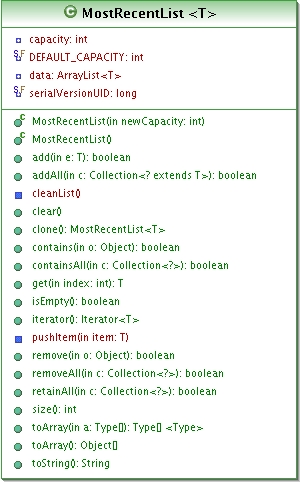
\includegraphics[scale=.5]{UMLMostRecentList.jpg}
  \caption[MostRecentlyUsedList]%
  {MostRecentlyUsedList\protect\footnotemark}
  \label{fig:MostRecentlyUsedList}
\end{figure}

\section{Preference pages}
\begin{itemize}
 \item place to easily configure settings, all KIELER preferences in one place
 \item integrated into eclipse look and feel
\end{itemize}

\subsection{Configuration page}
\begin{itemize}
 \item changing default configuration for internal properties
 \item check boxes for changing visibility of the combos
\end{itemize}

\subsubsection{User defined properties page}
\begin{itemize}
 \item adding/removing properties
 \item modified from msp, table view with providers
\end{itemize}

\subsubsection{Property usage dialog}
This dialog shown in figure \ref{fig:PropertyUsageDialog} is used for selecting which properties should always be taken
from the default configuration rather than the configuration component contained
in every .execution file.
The dialog used for this is a ListSelectionDialog which just receives the list of
all keys as input and the list of PropertyKeys from the PropertyUsageManager as default selection.
After the user is finished with selecting attributes and hit the 'Ok' Button the dialog
passes the new list of selected items back to the PropertyUsageManager.
\begin{figure}[PropertyUsageDialog]
  \centering
  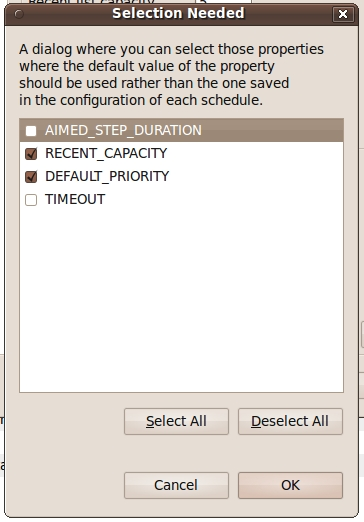
\includegraphics[scale=.5]{PropertyUsageDialog.jpg}
  \caption[Property Usage Dialog]%
  {The Property Usage Dialog\protect\footnotemark}
  \label{fig:PropertyUsageDialog}
\end{figure}

\subsection{Scheduling page}
This preference page is used to manage the schedules and the editors that they belong to.
This page is basicly a modified version of the LayoutPrioritiesPage by msp.

\begin{itemize}
 \item table with schedules / editors and their priorities
 \item modified from msp , editors = diagram types, schedules = layouters
 \item modify priorities
 \item add/remove editors, remove schedules, selecting default editor
\end{itemize}

\subsubsection{Adding and removing editors, Selecting a default editor}
On the scheduling preference page there are routines for adding and removing
editors as well as selecting a default editor.
All of these actions use the same basic method for displaying an ElementListSelectionDialog \ref{fig:EditorSelectionDialog}
that takes a list of editor ids and returns the one selected by the user.
\begin{itemize}
 \item The editor adding dialog gets a list of all editors currently registered on the
 active workbench. The user can select a single editor which is then added to the table.
 \item The editor removal dialog gets a list of all editors currently available for 
 assignment of support properties. The editor selected by the user is removed from the table.
 It is also removed from all schedules. This is done to prevent the schedule objects from growing
 to monstrous size over time when editors are getting added and removed.
 \item The default editor selection dialog gets the same list as the removal dialog. The selected
 editor is then set as default editor. The default editor is used when there is no currently active editor on the workbench.
  It is used:
  \begin{enumerate}
   \item to determine which editors to show in the Matching combo box.
   \item when a new schedule is created as an editor id.
  \end{enumerate}
\end{itemize}
\begin{figure}[EditorSelectionDialog]
  \centering
  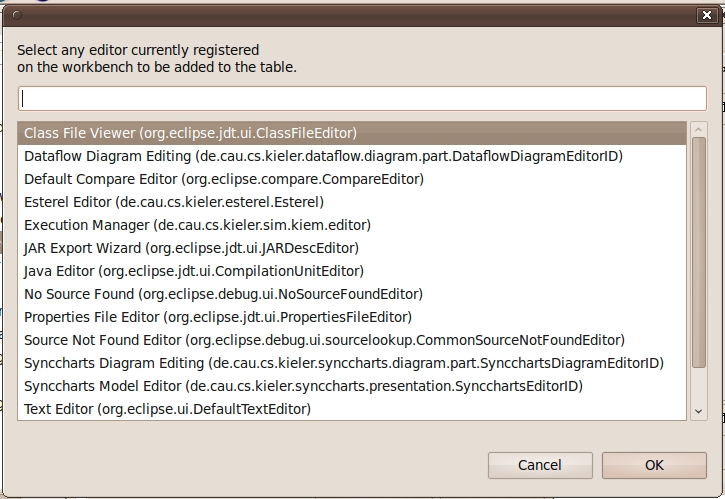
\includegraphics[width=1\textwidth]{EditorSelectionDialog.jpg}
  \caption[Editor Selection Dialog]%
  {The Editor Selection Dialog\protect\footnotemark}
  \label{fig:EditorSelectionDialog}
\end{figure}